\section{LIME}

LIME \cite{ribeiro2016should} is a black box interpretability method. Like all black box methods, LIME randomly changes features in the input data to detect which feature is relevant for the classification. The output of LIME is a list of features which the algorithm detected as to be relevant for the classification, sorted by importance.

In the case of image classification, LIME does not modify single pixels, because this would generate too many different versions of the input.
Instead, LIME generates superpixels.

\begin{figure}[H]
\centering
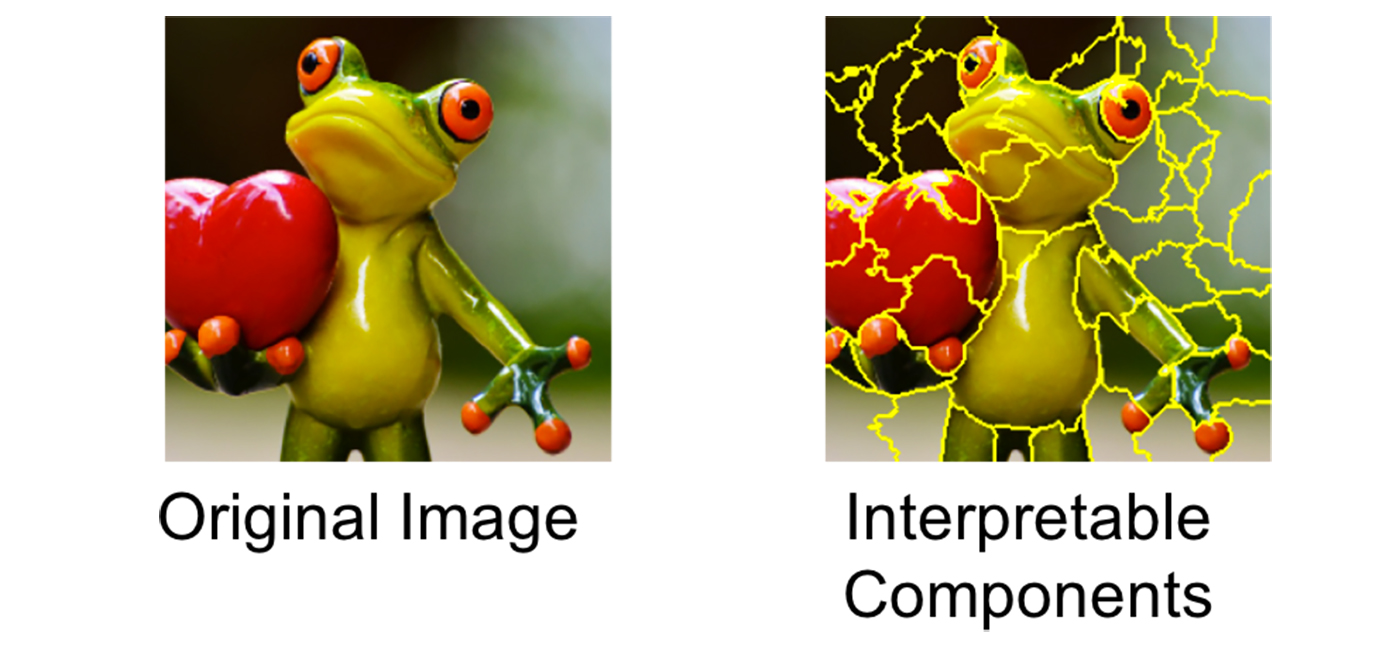
\includegraphics[width=12cm]{chapters/02_methods/images/lime.jpg}
\caption{Superpixels generated for an input image. Superpixels are the features LIME analyzes to detect if they are relevant for the classification.\cite{limeoreilly}}
\label{lime_superpixel}
\end{figure}

Superpixels are continuous regions on an image with a similar color. In the Python reference implementation, LIME uses the Quick Shift \cite{vedaldi2008quick} clustering algorithm to generate these superpixels. Figure \ref{lime_superpixel} shows superpixels overlaid on an example image.

In the next step, LIME generates input images by turning off multiple randomly selected superpixels. Turning off in this case means settings the color inside the superpixel to gray. Figure \ref{lime_perturbed} shows some examples of deactivated superpixels. The generated input images are then run trough the neural network and the new probabilities of the relevant class are recorded. 
As a last step, LIME does a locally weighted (i.e. adjacent superpixels are weighted higher) regression of the probabilities to generate a preferably continuous cluster of superpixels explaining a specific class.

\begin{figure}[H]
\centering
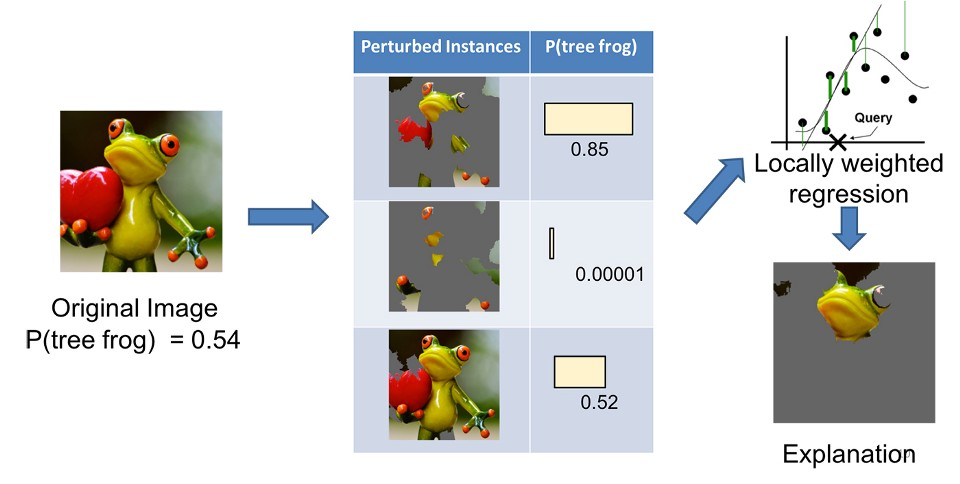
\includegraphics[width=14cm]{chapters/02_methods/images/lime2.jpg}
\caption{Left: Original image with detected class and probability. Middle: Perturbed images by randomly turned off superpixels and their probability for the specific class.
Right: Locally weighted regression to generate a preferably continuous region to explain the class.\cite{limeoreilly}}
\label{lime_perturbed}
\end{figure}

Figure \ref{lime_dog} 

\begin{figure}[H]
\centering
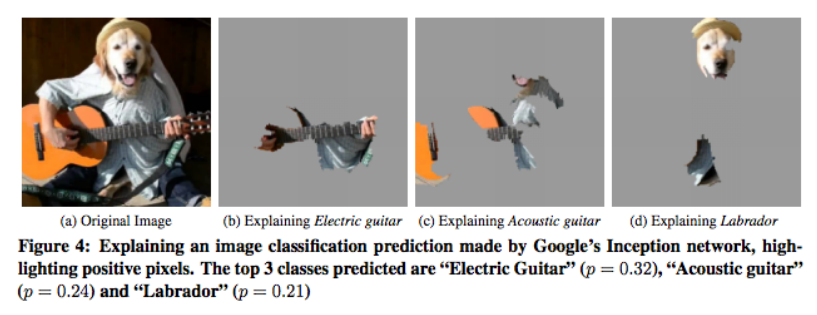
\includegraphics[width=14cm]{chapters/02_methods/images/lime.png}
\caption{Image from original LIME paper explaining three classes for the same input image.}
\label{lime_dog}
\end{figure}
